\chapter{Reconstruction rapide de structures cristallines}
\label{ch-chapter_4}
\dochaptoc
%
\section{Contexte général}

\subsection{Description des images STEM-EELS de structures cristallines}

Les images haute résolution déjà présentées à la \cref{sec-prop-eels} sont acquises sur des échelles restreintes (typiquement une dizaine de nanomètres) afin de visualiser les colonnes atomiques de l'échantillon. 
%
Contrairement aux données basse résolution détaillées à la section~\ref{sec-donnees-sous-echantillonnees}, la résolution de l'image n'est pas limitée par l'expérimentateur en vue de préserver l'échantillon mais par le pouvoir séparateur du microscope. On dit alors que l'image est \emph{haute résolution}. Comme détaillé à la section~\ref{sec-positionnement-these}, le pouvoir séparateur du VG-HB501 (resp. du Nion UltraSTEM 200) dont dispose le LPS est de l'ordre du nanomètre (resp. du dixième de nanomètre). Pour imager les colonnes atomiques, le Nion UltraSTEM 200 est donc préféré.

Dans le cadre applicatif de ce chapitre, nous étudierons les structures spatialement périodiques, comme les réseaux cristallins dont un exemple d'image HAADF est donné à la figure~\ref{fig-chap2-haadf-ex-b}. Acquérir ce type de structure nécessite d'orienter correctement le réseau cristallin. 
%
Comme détaillé à la section~\ref{sec-ech-sensibles}, les acquisitions haute résolution sont particulièrement sensibles aux distorsions liées à l'acquisition. En particulier, la dérive de l'échantillon peut déformer le réseau cristallin, comme le montre la figure~\ref{fig-drift}.

%\begin{figure}[b]
%    \centering
%    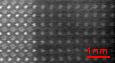
\includegraphics[width=0.4\textwidth]{img/chapitre1/figure4/haadf-HR-sc.png}
%    %
%    \caption{\protect\label{fig-chap4-HR-crist}Exemple d'image HAADF haute résolution d'une structure cristalline.}
%\end{figure}



\subsection{Parcimonie groupée dans une base choisie}

Le chapitre~\ref{ch-chapter_2} concluait sur l'intérêt de l'approche par \gls{mc} régularisés pour élaborer une technique de reconstruction rapide et performante et le chapitre~\ref{ch-chapter_3} proposait de telles méthodes pour traiter des images spatialement lisses, reposant sur une régularisation de Sobolev. 
%
Dans le cadre de ce chapitre, une méthode par \gls{mc} régularisés est également envisagée pour répondre aux contraintes en temps et en performances et une régularisation appropriée aux images haute résolution d'échantillons cristallins spatialement périodiques est requise.
%
Puisque les image haute résolution présentent des contours plus marqués que pour les images basse-résolution, un premier choix pourrait être la régularisation TV qui conserve mieux les contours que Sobolev. Cependant, cette régularisation ne tire pas parti de la redondance spatiale induite par le réseau cristallin, ce qui est une information a priori forte, et une méthode non-locale sous forme variationelle comme celles décrites à la section~\ref{sec-art-patch} peut être envisagée. Toutefois, plus que la redondance spatiale, c'est la \emph{périodicité} du réseau cristallin qui constitue la source d'information la plus forte. C'est pourquoi une méthode par \gls{mc} régularisés exploitant la parcimonie dans une base appropriée sera préférée dans ce chapitre. 

En particulier, afin de respecter les contraintes en temps de calcul, cette base ou dictionnaire peut être choisi a priori en exploitant des propriétés attendues concernant les images à reconstruire. Apprendre ce dictionnaire durant une étape de pré-traitement serait trop long pour notre application et les performances de reconstruction dépendraient fortement des données d'entraînement. Par conséquent, une base analytique tel que la base de Fourier, la \gls{dct} ou les ondelettes seront préférées pour leur expression explicite. Le choix de cette base sera discuté à la section~\ref{sec-appropriate-basis} en se basant sur des expériences.
%
Cependant, la base optimale serait celle qui minimiserait le nombre de coefficients non nuls dans cette base~; et en considérant la structure périodique des réseaux cristallins, cela devrait favoriser les bases périodiques, comme la base de Fourier ou la base \gls{dct}. 

Plus précisément, dans le cas de spectre-images EELS de réseaux cristallins, chaque image 2D obtenue pour une certaine perte d'énergie est censée présenter un motif périodique pouvant être décrit par une représentation parcimonieuse dans une base appropriée. Au contraire, chaque spectre mesuré en une position spatiale quelconque a peu de chance de présenter une périodicité particulière. Ainsi, cette propriété de parcimonie ne tient que dans les directions \emph{spatiales} du cube de donnée 3D.
%
De plus, il est légitime de penser que les représentations dans une même base de ces images 2D partagent des caractéristiques communes puisque la structure spatiale est probablement la même dans tous les canaux et ne dépend que de l'échantillon. Pour à la fois exploiter cette propriété de parcimonie et favoriser cette structure spatiale commune à travers les bandes, nous utiliserons une régularisation basée sur une parcimonie groupée, qui tend à promouvoir les spectre-images dont les coefficients non-nuls de représentations
associés à chaque bande sont localisés au même endroit endroit.
%
Ce phénomène est illustré à la figure~\ref{fig-joint-sparsity} en considérant une représentation dans la base \gls{dct} (le choix de cette base sera discuté à la section~\ref{sec-appropriate-basis}).
\begin{figure}[t]
    \centering
    \begin{tabular}{ccc}
    &Image&DCT seuillée\\
    %
    \rotatebox{90}{HAADF}&
    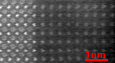
\includegraphics[width=0.4\textwidth]{img/chapitre4/figure1/haadf_size.png}&
    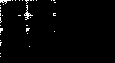
\includegraphics[width=0.4\textwidth]{img/chapitre4/figure1/haadf_th.png}\\[20pt]
    %
    \rotatebox{90}{Bande \num{} \np{1047}}&
    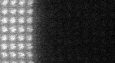
\includegraphics[width=0.4\textwidth]{img/chapitre4/figure1/spim_0.png}&
    
\includegraphics[width=0.4\textwidth]{img/chapitre4/figure1/spim_0_th.png}\\[20pt]
    %
    \rotatebox{90}{Bande \num{} \np{1111}}&
    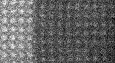
\includegraphics[width=0.4\textwidth]{img/chapitre4/figure1/spim_1.png}&
    
\includegraphics[width=0.4\textwidth]{img/chapitre4/figure1/spim_1_th.png}\\[20pt]
    %
    \rotatebox{90}{Bande \num{} \np{1451}}&
    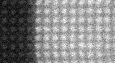
\includegraphics[width=0.4\textwidth]{img/chapitre4/figure1/spim_2.png}&
    
\includegraphics[width=0.4\textwidth]{img/chapitre4/figure1/spim_2_th.png}\\
\end{tabular}
    \caption{\protect\label{fig-joint-sparsity}
        Illustration de la parcimonie groupée présente dans les données EELS. L'acquisition STEM est composée d'une image 2D HAADF  (1\textsuperscript{ère} ligne à gauche) et du spectre-image correspondant dont trois bandes sont considérées (lignes 2 à 4, colonne de gauche). Pour chaque image, la répartition des 2\% coefficients de plus grande valeur absolue est représentée (colonne de droite). 
        %
        \`A noter que la plupart de ces coefficients sont situés dans les mêmes zones de l'espace \gls{dct} que ce soit pour l'image HAADF ou pour les bandes du spectre-image, ce qui suggère une certaine parcimonie groupée dans l'espace transformé.}
\end{figure}
Notons que dans le cas d'un niveau de bruit important, comme c'est le cas pour la bande \num{} \np{1111}, certains coefficients puissants assimilés aux hautes fréquences correspondent au bruit (dans le coin inférieur droit des représentations). Cependant, en analysant conjointement les représentations dans la base \gls{dct} pour plusieurs bandes, la disposition des coefficients principaux peut être déterminée après soustraction des coefficients associés au bruit.

\newpage
%
\section{La méthode CLS}

\subsection{Formulation}\label{sec-formulation-cls}

En se basant sur l'état de l'art mené au chapitre~\ref{ch-chapter_2} et sur les choix de la section précédente, la méthode proposée repose sur un problème de \gls{mc} régularisés s'écrivant 
\begin{equation}\label{eq-cls-formulation}
    \gls{Xh}=\argmin_{\gls{X}} \frac{1}{2} \frobnorm{\gls{Yi} - \gls{X}_{\gls{I}}} + \gls{lcls} \mathcal{R}(\gls{X})
\end{equation}
où l'opérateur $\mathcal{R}(\cdot)$ est une régularisation et où \gls{lcls} est un scalaire ajustant l'importance de la régularisation par rapport au terme d'attache aux données. Afin de contraindre le motif spatial périodique à être similaire pour l'ensemble des canaux, la régularisation choisie est
\begin{equation}\label{eq-regul-cls}
    \mathcal{R}(\gls{X}) = ||\gls{X}\boldsymbol\Psi||_{2, 1}
\end{equation}
où $\boldsymbol\Psi$ est un opérateur orthogonal appliquant un changement de base de manière bande à bande. La norme $\ell_{2, 1}$ est définie comme~\cite{kowalski2009sparse}%
\begin{equation}
||\mathbf{U}||_{2, 1} = \sum_j||\mathbf{U}_j||_2 = \sum_j \sqrt{\sum_i |\mathbf{U}_{ij}|^2}.
\end{equation}
Minimiser cette norme permet de contraindre la parcimonie groupée puisque qu'elle tend à annuler les colonnes de faible énergie tout en conservant celles dont l'énergie est maximale, et dans ce cas, tous les coefficients sont non-nuls. Dans le cas d'une base périodique (\eg\ Fourier ou \gls{dct}), la régularisation~\eqref{eq-regul-cls} promeut des représentations fréquentielles similaires et parcimonieuses pour l'ensemble des bandes. Dans la suite, cette technique sera appelée \gls{cls}.

\gls{cls} peut être directement appliquée au spectre partiellement acquis, comme nous le verrons à l'annexe~\ref{sec-perfs-without-acp}. Cependant, de même que pour la méthode \gls{3s}, nous proposons de conduire une \gls{acp} sur les données acquises \gls{Yi} et d'appliquer \gls{cls} aux $R$ composantes principales les plus puissantes.
%
La formulation~\eqref{eq-cls-formulation} reste la même, mais la matrice d'observation \gls{Yi} et l'image reconstruite \gls{X} sont remplacées par leur équivalent dans le domaine de l'\gls{acp}, à savoir resp. $\gls{H}_{1:\gls{R}}^T\gls{Yi}$ et \gls{S}. L'image reconstruite complète \gls{X} peut être obtenue de \gls{S} en appliquant la transformation inverse, à savoir $\gls{X} = \gls{H}_{1:\gls{R}}\gls{S}$. Si cette étape n'est pas une condition préalable à la méthode, elle présente plusieurs avantages déjà discutés à la section~\ref{subsec-formulation-3s} concernant \gls{3s}.
%
D'abord, cela introduit explicitement une régularisation spectrale au problème d'inpainting en imposant la structure faible rang de la solution. Des stratégies similaires ont été largement utilisées pour différentes tâches dans le cadre des images multibandes, entre autres l'acquisition comprimée~\cite{zhang2011joint, martin2014hyca}, l'inpainting~\cite{shuang2018fast}, la fusion~\cite{wycoff2013nonnegative,simoes2014convex,wei2015fast} ou l'analyse de mélanges~\cite{dobigeon2009joint,dobigeon2012spectral}.
%
Ensuite, réduire la taille des données à traiter permer de diminuer significativement le temps d'exécution.
%
Ce pré-traitement peut cependant induire quelques artefacts au cours de la reconstruction lorsque l'estimation de la matrice de covariance est imprécise, \eg\ dans le cas d'un taux d'échantillonnage faible. De plus, comme expliqué pour \gls{3s}, le nombre $R$ de composantes principales à conserver (cette valeur correspondant à la dimension du sous-espace signal sera appelé le \emph{seuil} de l'ACP dans la suite) devra être attentivement choisi puisque un seuil trop petit peut faire disparaître des structures de faible puissance~\cite{mevenkamp2017mm}. Deux stratégies pour ajuster ce seuil sont proposées à la section~\ref{subsec-3s-poids} et à l'annexe~\ref{sec-spim-creation-hr}. La pertinence de l'utilisation de l'ACP comme pré-traitement est discutée à l'annexe~\ref{sec-perfs-without-acp}.
%
Pour alléger l'écriture, la suite de la présentation sera faite avec les notations $\mathbf{Y}$ et $\mathbf{X}$ associées au problème formulé dans l'espace initial.

\subsection{Choix du paramètre \gls{lcls}}\label{sec-choix-param-CLS}

Le choix du paramètre de régularisation \gls{lcls} dans~\eqref{eq-cls-formulation} est non-trivial pour un problème inverse dans le cas général. Toutefois, il peut être ajusté de manière acceptable en exploitant l'information a priori disponible pour l'image à reconstruire, comme le niveau de bruit (pouvant être estimé en amont) ou le niveau de parcimonie, \ie{}, la proportion de coefficients non-nuls de la représentation.
%
De même que dans la section~\ref{sec-s2n-param-tuning} pour S2N, cette connaissance a priori peut être utilisée pour évaluer la qualité de la reconstruction $\gls{Xh}_{\gls{lcls}}$ obtenue avec CLS pour une paramètre de régularisation $\gls{lcls}$ donné. Par exemple, pour une solution pertinente, le terme d'attache aux données doit être de l'ordre de grandeur du niveau de bruit. Une recherche dichotomique peut alors être conduite afin d'ajuster automatiquement le paramètre de régularisation. En d'autres termes, CLS est executé pour une valeur de paramètre donnée et le terme d'attache aux données est évalué à la convergence. Puisque le terme d'attache aux données croît avec \gls{lcls}, si sa valeur est inférieure (resp. supérieure) au niveau de bruit, \gls{lcls} devra être augmenté (resp. diminué) et CLS devra être de nouveau exécuté. Cette stratégie est testée à l'annexe~\ref{sec-lcls-param-estim} en se basant sur une image semi-réelle.

\subsection{Implémentation}

Reconstruire le spectre-image \gls{X} complet à partir de \gls{Yi} peut être formulé selon le problème d'optimisation suivant
\begin{equation}
\gls{Xh}=\argmin_{\gls{X}} 
    \underbrace{\frac{1}{2} \frobnorm{\gls{Yi} - \gls{X}_{\gls{I}}}}_{f(\gls{X})} +
    \underbrace{ \gls{lcls} ||\gls{X}\boldsymbol\Psi||_{2, 1}}_{g(\gls{X})}.
\end{equation}
Ce problème d'optimisation peut être facilement résolu à l'aide de l'algorithme FISTA décrit à la section~\ref{sec-fista}. Pour cela, seuls trois éléments doivent être évalués, à savoir le gradient $\nabla f$, une borne supérieure $L$ de la constante de Lipschitz $L(f)$ de $\nabla f$ et l'opérateur proximal  $\mathrm{prox}_{g}(\gls{X})$. La fonction gradient $\nabla f$ s'écrit facilement comme suit
\begin{equation}
    \nabla f(\gls{X}) = (\gls{X}\gls{Phi} - \gls{Yi})\gls{Phi}^T
\end{equation}
où $\gls{Phi}$ est l'opérateur de sous-échantillonnage tel que $\gls{X}_{\gls{I}} = \gls{X}\gls{Phi}$. La constante de Lipshitz associée vaut
\begin{equation}
    L(f) = ||\nabla^2 f(\gls{X})|| = ||\gls{Phi}\gls{Phi}^T|| = 1.
\end{equation}
Enfin, l'opérateur proximal est séparable suivant les colonnes, et est évalué en réalisant un seuillage doux pour toute colonne $\mathbf{x}_j$ (avec $j=1, \dots, P$) selon~\cite{jenatton2011proximal}
\begin{equation}
[\mathrm{prox}_{\mu g}(\gls{X})]_j = 
\begin{cases}
0&\text{si}\ ||\mathbf{x}_j||_2 < \mu \gls{lcls}\\
\left(1-\frac{\mu\gls{lcls}}{||\mathbf{x}_j||_2}\right)\mathbf{x}_j&\text{sinon}\\
\end{cases}.\label{eq-prox-op}
\end{equation}
Comme expliqué à la section~\ref{sec-formulation-cls}, la méthode de reconstruction peut être appliquée à la matrice d'observation \gls{Yi} ou à sa représentation $\gls{H}_{1:\gls{R}}^T\gls{Yi}$ dans un sous-espace de dimension réduite identifié par ACP. Le seuil $R$ à fixer peut être choisi en suivant les stratégies décrites à la section~\ref{subsec-3s-poids} et à l'annexe~\ref{sec-spim-creation-hr}.



\subsection{La méthode DL-CLS}

Comme nous le verrons à la section~\ref{sec-hr-results}, l'algorithme CLS reconstruit rapidement et efficacement le spectre-image à partir de données partiellement acquises. Par conséquent, cette section propose d'appliquer CLS comme pré-traitement à des techniques plus avancées, en particulier pour initialiser les méthodes par \gls{ad}. Pour cela, les données reconstruites par CLS sont décomposées en un dictionnaire et en une représentation parcimonieuse à l'aide de l'algorithme conventionnel mini-batch proposé dans~\cite{mairal2009online} couplé à OMP~\cite{mallat1993matching, pati1993orthogonal} (\cf{} section~\ref{sec-art-patch}). Ces dictionnaires et codes sont ensuite utilisés comme initialisation pour les approches par \gls{ad}.
%
Cette technique d'initialisation nommée DL-CLS est particulièrement intéressante pour \gls{wksvd} et ITKrMM qui résolvent un problème d'optimisation non-convexe basé sur un schéma de directions alternées. En effet, pour de tels problèmes non-convexes, l'initialisation est un problème crucial pour s'assurer de converger vers une solution pertinente.
%
Par contre, une stratégie similaire ne peut être adoptée pour initialiser BPFA puisque cette technique implémente un algorithme de \gls{mcmc} et que les distributions des codes et du dictionnaire dépendent de la distribution des hyperparamètres.
%
La pertinence de CLS comme technique d'initialisation sera discutée à la section~\ref{sec-DL-CLS}.

%
\section{Expériences}\label{sec-experiments-hr}

\subsection{Données}\label{sec-donnees-hr}

\paragraph{Données réelles.} Deux spectre-images réels notés $\mathsf{R}_1$ et $\mathsf{R}_2$ ont été acquis sur le Nion UltraSTEM200 au LPS. 
%
$\mathsf{R}_1$ est un spectre-image acquis à 100\;kV à partir d'une hétéro-structure $\mathrm{La}_{1‐\mathrm{x}}\mathrm{Sr}_{\mathrm{x}}\mathrm{MnO}_3$/$\mathrm{Pb}(\mathrm{Zr,Ti})\mathrm{O}_3$ (LSMO/PZT) reposant sur un composé $\mathrm{SrTiO}_3$~\cite{li2016charge}. Les spectres ont été échantillonnés sur une gamme d'énergie correspondant aux seuils $\mathrm{Ti-L}_{2,3}$, $\mathrm{O-K}$, $\mathrm{Mn -L}_{2,3}$ et $\mathrm{La-M}_{4,5}$.
%
$\mathsf{R}_2$ est un spectre-image acquis à 100\;kV à partir d'un film fin de $\mathrm{NdNiO}_3$ sur un substrat de $\mathrm{LaAlO}_3$~\cite{preziosi2018direct}. Les spectres ont été acquis sur une gamme correspondant aux seuils de $\mathrm{O-K}$, $\mathrm{La-M}_{4,5}$, $\mathrm{Ni-L}_{2,3}$ et $\mathrm{Nd-M}_{4,5}$.
%
Pour réduire le bruit d'acquisition, les images ont été acquis avec un temps d'exposition relativement long. Des informations complémentaires concernant ces images (comme leur taille, leur résolution, leur temps d'exposition et le seuil de l'ACP $R$ utilisé à la section~\ref{sec-results-hr-synth}) sont reportées à la \tabname~\ref{table-hr-samples}.

Toutes les expériences discutées dans la section suivante~\ref{sec-hr-results} sont réalisées sur un CPU Intel Xeon E5540 @ 2,53\,GHz avec 8 c\oe{}urs (en incluant l'hyperthreading) et sur une mémoire de 50\,Gb. \`A noter que seul BPFA requiert une telle mémoire, les autres méthodes peuvent fonctionner avec seulement 13.2\,Gb de mémoire.

\begin{table*}
    \centering
    \setlength\tmplength{2.5cm}
\bgroup
    \renewcommand{\arraystretch}{1.2}
    \begin{tabular}{%
            c%
            M{\tmplength}%
            m{1.3\tmplength}%
            M{1.9cm}%
            c%
            c%
            M{2cm}}%
        \toprule
        \multirow{2}*{Image}& 
        \multirow{2}*{Echantillon}& 
        \multirow{2}{1.3\tmplength}{%
            {Taille ($x$, $y$, $\lambda$)\newline Res. ($\Delta x = \Delta y$, $\Delta \lambda$)}}&
        \multirow{2}{0.7\tmplength}{%
            \centering\arraybackslash Temps d'exp. (ms)}&
        \multicolumn{2}{c}{Seuils d'intérêt}&
        \multirow{2}{2cm}{\centering\arraybackslash Seuil de l'ACP $R$}\\
        %\cline{5-7}
        &&&&\'Elément&Perte d'éner. (eV)&\\
        \midrule
        %
        %
        \multirow{4}*{$\mathsf{R}_1$}& % Name
        \multirow{4}{\tmplength}{\centering\arraybackslash 
                      PbZrTiO\textsubscript{3} / 
                      LaSrMnO\textsubscript{3} / 
                      SrTiO\textsubscript{3}
                      }& % Sample
        \multirow{4}{1.3\tmplength}{(232, 101, 1530)\newline{(\np[nm]{0.055}, \np[eV]{0.27})}}& % Shape
        \multirow{4}*{20}& % Dwell time
        Ti& % Element
        456& % eV
        \multirow{4}*{9}\\ % PCA th
        %
        &&&&O& 532&\\
        &&&&Mn& 640&\\
        &&&&La& 832&\\
        \midrule
        %
        %
        \multirow{4}*{$\mathsf{R}_2$}& % Name
        \multirow{4}{\tmplength}{\centering\arraybackslash 
                      NdNiO\textsubscript{3}/
                      LaAlO\textsubscript{3}
                      }& % Sample
        \multirow{4}{1.3\tmplength}{(63, 115, {1505}){\newline(\np[nm]{0.045}, \np[eV]{0.32})}}& % Shape
        \multirow{4}*{20}& % Dwell time
        O& % Element
        532& % eV
        \multirow{4}*{7}\\ % PCA th
        %
        &&&&La& 832&\\
        &&&&Ni& 855&\\
        &&&&Nd& 978&\\
        \midrule
        %
        %
        $\mathsf{S}$& % Name
        cf. $\mathsf{R}_2$& % Sample
        (70, 120, 1435){\newline(\np[nm]{0.045}, \np[eV]{0.32})}& % Shape
        -& % Dwell time
        \multicolumn{2}{c}{cf. $\mathsf{R}_2$}&
        4\\ % PCA th
        \bottomrule
    \end{tabular}
\egroup
    \caption{Informations complémentaires sur les images $\mathsf{R}_1$, $\mathsf{R}_2$ et $\mathsf{S}$
        \protect\label{table-hr-samples}
    }
\end{table*}

\paragraph{Images synthétiques et semi-réelles.} Puisque $\mathsf{R}_1$ et $\mathsf{R}_2$ sont naturellement corrompues par un bruit, le calcul de métriques pertinentes en vue d'évaluer la performance des techniques de reconstruction risque d'être biaisé par un niveau de bruit inconnu. Pour contourner le problème, des versions débruitées de $\mathsf{R}_1$ et $\mathsf{R}_2$ ont d'abord été générées en appliquant une ACP et en ne conservant que les $R$ premières composantes principales. Le choix du seuil $R$ est, de manière générale, une tâche difficile. Dans ce chapitre, il a été fixé de sorte que les composantes principales supprimées ne contiennent pas d'information spatiale. Pour quantifier la présence ou l’absence d’information spatiale dans une composante principale, la blancheur du bruit résiduel est évaluée en se basant sur les métriques proposées dans~\cite[chap. 3]{riot2018residual}. Plus de détails sont donnés à l'annexe~\ref{sec-spim-creation-hr}. Ces images débruitées, notées $\bar{\mathsf{R}}_1$ et $\bar{\mathsf{R}}_2$, sont supposées être les images vérité terrain \gls{X} à reconstruire.

En plus de ces deux images semi-réelles, un spectre-image synthétique a été généré à partir de l'image $\mathsf{R}_2$. Pour cela, une \gls{aci} a été appliquée à $\mathsf{R}_2$ afin d'extraire quatre spectres caractéristiques qui ont été filtrés ensuite, tandis que les cartes d'abondance associées ont été synthétiquement produites. Ces données ont été mélangées par la suite  afin d'obtenir le spectre-image noté $\mathsf{S}$ (\cf{} annexe~\ref{sec-spim-creation-hr} pour plus de détails concernant la construction de ces données).

Afin de simuler des conditions expérimentales, les trois images verité terrain $\bar{\mathsf{R}}_1$, $\bar{\mathsf{R}}_2$ et $\mathsf{S}$ ont été ensuite corrompues par un bruit blanc additif gaussien de sorte que le SNR soit réaliste%
%
\footnote{La reconstruction dans le cas d'un bruit mixte poisson-gaussien est discutée à l'annexe~\ref{sec-bruit-mixte} en se basant sur des expériences semblables à celles menées à la section~\ref{sec-results-hr-synth}.}%
%
. Enfin, ces images pseudo-réelles, notées $\mathsf{R}_1^*$ et $\mathsf{R}_2^*$, et l'image synthétique bruitée $\mathsf{S}^*$, ont été spatialement et aléatoirement sous-échantillonnées suivant une loi uniforme avec un taux d'échantillonnage de 20\% en vue de produire la matrice d'observation \gls{Yi}. Notons que les résultats obtenus pour d'autres taux d'échantillonnage sont donnés à l'annexe~\ref{sec-autres-taux-echantillonnage-hr}. 

\subsection{Méthodes}

Comme expliqué à la section~\ref{sec-formulation-cls}, pour l'ensemble des algorithmes, une ACP est d'abord appliquée à l'image observée en ne conservant que les $R$ premières composantes les plus puissantes. Les techniques de reconstruction sont ensuite appliquées dans cet espace de dimension réduite. La transformation inverse sera réalisée en post-traitement pour obtenir l'image reconstruite \gls{Xh}. Les méthodes comparées sont NN, 3S, CLS, ITKrMM, \gls{wksvd} et BPFA. En particulier, NN est la seule à être appliquée bande à bande. Pour toutes les techniques, les paramètres de l'algorithme ont été ajustés afin d'atteindre les performances optimales. En particulier, les techniques par \gls{ad} considèrent des patchs 3D de taille $w\times w \times R$ avec $w=25$ pour ITKrMM et \gls{wksvd} et $w=41$ pour BPFA. Les métriques utilisées en vue de comparer ces techniques sont données à la section~\ref{sec-metriques}.

Les implémentations de ITKrMM et de \gls{wksvd} utilisées dans ces expériences sont les codes Matlab fournis par la Prof. K. Schnass\footnote{\url{https://www.uibk.ac.at/mathematik/personal/schnass/code/itkrmm.zip}}. L'implémentation de BPFA est le code Matlab fournit par le docteur Z. Xing\footnote{\url{https://drive.google.com/open?id=0B9548VKFKtmiY2ZNRFVUTjhyUFE}}. J'ai implémenté les autres méthodes ;  elles sont disponibles sous la forme d'une librairie Python que j'ai créée nommée \texttt{inpystem}\footnote{\url{https://github.com/etienne-monier/inpystem}}. Les codes permettant de reproduire certaines des expériences de ce chapitre sont également disponibles en ligne\footnote{\url{https://github.com/etienne-monier/2020-Ultramicro-fast}}.



%
\section{Résultats}\label{sec-hr-results}

\subsection{Base appropriée pour la parcimonie}\label{sec-appropriate-basis}

Comme expliqué à la section précédente, le niveau de parcimonie des données dépend grandement de l'image et de la base choisie pour sa représentation. Dans le cas d'images de réseaux cristallins à échelle atomique, des travaux précédents ont considéré les ondelettes~\cite{li2018compressive}, la base de Fourier~\cite{stevens2018apl} ou la base \gls{dct}~\cite{beche2016development,anderson2013sparse}. Toutefois, aucune comparaison systématique de ces transformations n'a été conduite dans ces travaux. Cette section propose de combler cette lacune. Intuitivement, les transformées de Fourier ou la \gls{dct} devraient donner les meilleurs résultats puisqu'elles sont connues pour donner des représentations très parcimonieuses dans le cadre de structures périodiques et lisses. 
%
Pour confirmer cette intuition, nous proposons de tracer l'erreur de reconstruction comme une fonction du ratio $r\in(0, 1)$ de coefficients de représentation non-nuls, \ie{}, en ne conservant seulement que les $r$\% coefficients de représentation dont la magnitude est la plus élevée. La transformation inverse fournit une estimée \gls{Xh} de \gls{X} d'autant dégradée que $r$ décroît. L'erreur de reconstruction correspond à la NMSE entre \gls{Xh} et \gls{X}. La transformation la plus appropriée à une image est celle dont l'erreur de reconstruction décroît le plus vite avec $r$ puisque cela signifie que l'on a besoin de moins de coefficients pour décrire l'image.
%la valeur absolue des coefficients de représentation qui doivent décroître aussi vite que possible quand ils sont triés par ordre décroissant. Une décroissance rapide de la courbe signifierait que l'on a besoin de moins de coefficients pour représenter précisément les données. 
%
Ainsi, l'erreur de reconstruction est évaluée pour chaque image et est représentée pour les transformées suivantes : la base de Fourier, la base \gls{dct}, les ondelettes de Daubechies et symlet%
%
\footnote{Le niveau maximal a été choisi pour la décomposition en ondelette. Plus précisément, la décomposition s'arrête lorsque l'image devient plus petite que la taille du filtre FIR utilisé pour la décomposition en ondelette du signal.} %
%
(avec 3, 10 et 20 moments nuls). 
%
% L'erreur de reconstruction est évaluée comme une fonction du ratio $r\in(0, 1)$ de coefficients de représentation non-nuls, \ie{}, en ne conservant seulement que les $r$\% coefficients de représentation dont la magnitude est la plus élevée. La transformation inverse fournit une estimée \gls{Xh} de \gls{X} d'autant dégradée que $r$ décroît. L'erreur de reconstruction correspond au NMSE entre \gls{Xh} et \gls{X}. Pour résumer, la transformation la plus appropriée à une image est celle dont l'erreur de reconstruction décroît le plus vite avec $r$ puisque cela signifie que l'on a besoin de moins de coefficients pour décrire l'image.

Cette procédure a été appliquée à $\mathsf{R}_1$, $\mathsf{R}_2$ et $\mathsf{S}$ après une ACP. Les résultats sont donnés à la figure~\ref{fig-best-basis}. Ils montrent que la base \gls{dct} est toujours meilleure que la base de Fourier puisque les mesures ont des valeurs réelles, ce qui introduit de la redondance avec un facteur 2 pour chaque axe dans l'espace de la transformée de Fourier 2D tandis que la base \gls{dct} ne subit pas cette redondance. De plus, notre intuition est confirmée puisque les bases \gls{dct} et Fourier sont les meilleures pour les trois images, comparé à toutes les transformations en ondelettes considérées. Finalement, dans le cas des images de réseaux périodiques étudiées dans ce chapitre, ces expériences montrent que la base \gls{dct} offre la représentation la plus parcimonieuse et c'est cette transformation bande à bande $\boldsymbol\Psi$ qui sera choisie dans~\eqref{eq-regul-cls} pour la méthode CLS proposée.

\begin{figure}[t]
    \centering
    \subfigure[$\mathsf{R}_1$]{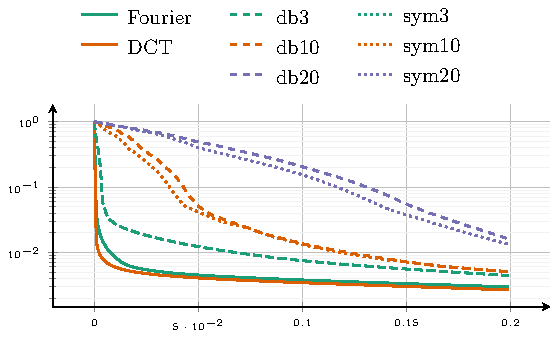
\includegraphics{img/chapitre4/figure3/best-basis-r1.pdf}}\\
    \subfigure[$\mathsf{R}_2$]{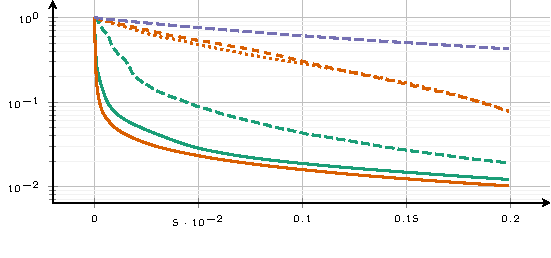
\includegraphics{img/chapitre4/figure3/best-basis-r2.pdf}}\\
    \subfigure[$\mathsf{S}$]{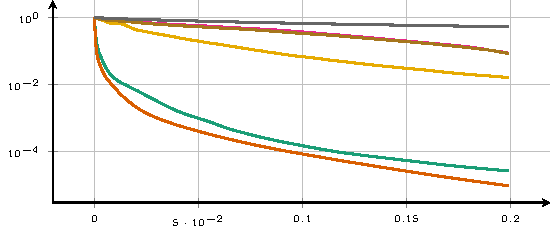
\includegraphics{img/chapitre4/figure3/best-basis-s.pdf}}\\
    \caption{Erreur de reconstruction (NMSE) en fonction de $r$. Différentes bases sont étudiées pour représenter $\mathsf{R}_1$ (en haut), $\mathsf{R}_2$ (au milieu) et $\mathsf{S}$ (en bas). Plus la courbe décroît rapidement, meilleur c'est puisque cela signifie que l'image a besoin de moins de coefficients pour être représentée précisément. La base \gls{dct} donne les meilleurs résultats pour toutes les images.
        \protect\label{fig-best-basis}}
\end{figure}





\subsection{Résultats sur les images synthétiques et semi-réelles}\label{sec-results-hr-synth}

Dans cette section, les techniques de reconstruction ont été appliquées aux deux images semi-réelles $\mathsf{R}_1^*$ et $\mathsf{R}_2^*$ et à l'image synthétique $\mathsf{S}^*$.

Les valeurs des métriques comme le temps d'exécution sont reportées à la \tabname~\ref{table-results-time-hr}. Ces résultats montrent qu'il y a un écart de performances très marqué, tant en termes de qualité que de temps d'exécution, entre NN et les méthodes par \gls{ad}. C'est particulièrement visible pour BPFA qui affiche un temps de calcul dépassant les 24 heures, mais qui offre souvent la meilleure reconstruction. Les techniques par \gls{mc} régularisés 3S et CLS semblent apporter un compromis, aussi bien en précision qu'en rapidité. CLS est particulièrement performante puisqu'elle affiche un SNR proche des meilleures méthodes avec un temps d'exécution très réduit. 3S affiche des performances plus faibles (même si supérieures à NN), ce qui est logique car la régularisation est inappropriée pour décrire précisément la structure périodique des images de réseaux cristallins. Notons également que BPFA donne généralement les meilleurs SNR et aSAD, à l'exception de $\mathsf{R}_1^*$ pour lequel CLS donne le meilleur aSAD tandis que NN affiche le aSAD le plus faible.

\begin{normalfigure*}[htbp]
    \centering
    \bgroup
    \renewcommand{\arraystretch}{1.2}
    
    \subfigure[$\mathsf{R}_1^*$]{
        \begin{tabular}{%
                c%
                c%
                c%
                c%
                c}%
            \toprule
            Méthode& 
            SNR&
            aSAD (100$\times$)&
            SSIM&
            Temps exec.(s)\\
            %
            \midrule
            %
	PPV & 30,81 & 1,384 & 0,680 & \textbf{0,423}\\
	3S & 32,30 & 1,080 & 0,643 & 15,2\\
	CLS & 36,18 & \textbf{1,061} & 0,912 & 18,4\\
	ITKrMM & 36,52 & 1,097 & 0,923 & $6,85\cdot 10^4$\\
	wKSVD & 36,93 & 1,091 & 0,931 & $7,97\cdot 10^4$\\
	BPFA & \textbf{37,02} & 1,089 & \textbf{0,933} & $1,36\cdot 10^5$\\
            \bottomrule
        \end{tabular}
    }\\[0.75cm]
    %
    \subfigure[ $\mathsf{R}_2^*$]{
        \begin{tabular}{%
                c%
                c%
                c%
                c%
                c}%
            \toprule
            Méthode& 
            SNR&
            aSAD (100$\times$)&
            SSIM&
            Temps exec.(s)\\
            %
            \midrule
            %
	PPV & 28,71 & 1,815 & 0,635 & $\mathbf{7,94\cdot 10^{-2}}$\\
	3S & 30,17 & 1,496 & 0,621 & 3,38\\
	CLS & 33,15 & 1,233 & 0,790 & 3,09\\
	ITKrMM & 33,67 & 1,253 & 0,819 & $9,55\cdot 10^3$\\
	wKSVD & 34,52 & 1,163 & 0,841 & $2,59\cdot 10^4$\\
	BPFA & \textbf{35,01} & \textbf{1,106} & \textbf{0,852} & $6,18\cdot 10^4$\\
            %
            \bottomrule
        \end{tabular}
    }\\[0.75cm]
    %
    \subfigure[ $\mathsf{S}^*$]{
        \begin{tabular}{%
                c%
                c%
                c%
                c%
                c}%
            \toprule
            Méthode& 
            SNR&
            aSAD (100$\times$)&
            SSIM&
            Temps exec.(s)\\
            %
            \midrule
            %
	PPV & 21,32 & 1,462 & 0,735 & $\mathbf{6,82\cdot 10^{-2}}$\\
	3S & 22,12 & 1,174 & 0,710 & 3,33\\
	CLS & 42,14 & 0,224 & 0,997 & 1,48\\
	ITKrMM & 44,16 & 0,338 & 0,998 & $9,61\cdot 10^3$\\
	wKSVD & 45,59 & 0,277 & 0,999 & $1,57\cdot 10^4$\\
	BPFA & \textbf{52,70} & \textbf{0,150} & \textbf{1,000} & $4,06\cdot 10^4$\\
            %
            \bottomrule
        \end{tabular}
    }\\[0.75cm]
\egroup
    \caption{Performances de reconstruction mesurées par SNR, aSAD et SSIM pour les images semi-réelles $\mathsf{R}_1^*$ et $\mathsf{R}_2^*$ et pour l'image synthétique $\mathsf{S}^*$. Le temps d'exécution est aussi donné pour être considéré conjointement avec la précision. Il y a un écart de performances très marqué tant en qualité qu'en temps d'exécution entre NN et les méthodes par \gls{ad}. Les méthodes par \gls{mc} régularisés forment un compromis, tout particulièrement CLS qui est plus performante que 3S.
        \protect\label{table-results-time-hr}}
\end{normalfigure*}

La reconstruction d'un pixel non échantillonné dont la position est donnée à la figure~\ref{fig-synth-image-spectra-locations} est aussi affichée à la figure~\ref{fig-synth-image-spectra}. Pour cette figure, les données de référence correspondent à l'image non bruitée $\bar{\mathsf{R}}_2$. Les courbes équivalentes pour un pixel échantillonné sont omises ici puisqu'elles n'apportent aucune information complémentaire, les spectres reconstruits étant trop proches pour être distingués.
%
Ces courbes montrent que le spectre reconstruit par NN est significativement décalé par rapport à la référence tandis que BPFA et CLS sont proches du spectre de référence. 

Les cartes d'erreur en NMSE sont représentées à la figure~\ref{fig-results-HR2_synth-bands}. Cette représentation peut être utile pour localiser les principales erreurs de reconstruction. De plus, la figure~\ref{fig-qu1-21-histograms} montre les histogrammes des erreurs pour chaque seuil. Ils montrent que l'erreur de NN est généralement supérieure par rapport aux autres méthodes, tout particulièrement pour certains pixels.

% Position pixel représenté
\begin{figure}[htbp]
    \centering
    %
    \subfigure[Bande \num\ 2 de $\bar{\mathsf{R}}_2$ \protect\label{subfig-location_samp}]{
        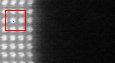
\includegraphics[height=0.25\textwidth]{img/chapitre4/figure5/rectangle.png}}\\
    %
    \subfigure[Bande \num\ 2 de $\bar{\mathsf{R}}_2$ (zoom) \protect\label{subfig-location_samp-zoom}]{
        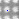
\includegraphics[height=0.2\textwidth]{img/chapitre4/figure5/zoom_rec.png}}\hskip 20pt
    %
    \subfigure[Masque (zoom) \label{subfig-location_samp-zoom-mask}]{
        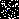
\includegraphics[height=0.2\textwidth]{img/chapitre4/figure5/zoom_rec_mask.png}}\\
    %
    \caption{Position du spectre échantillonné représenté à la figure~\protect\ref{fig-synth-image-spectra}.
        L'image \subref{subfig-location_samp} montre la seconde composante principale de l'image semi-réelle $\bar{\mathsf{R}}_2$. Le pixel bleu indique la position du spectre affiché à la figure~\protect\ref{fig-synth-image-spectra}. Les figures~\protect\subref{subfig-location_samp-zoom} et  \protect\subref{subfig-location_samp-zoom-mask} montrent un zoom de l'image sur la région d'intérêt et sur le masque d'échantillonnage. Les pixels blancs du masque d'échantillonnage correspondent à des pixels échantillonnés.
        \protect\label{fig-synth-image-spectra-locations}}
\end{figure}

% Pixel représenté
\begin{normalfigure*}[htbp]
    \centering
    %
    \subfigure[Pixel non-acquis]{
        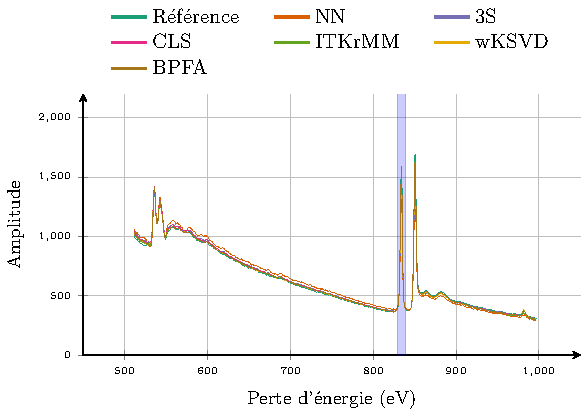
\includegraphics{img/chapitre4/figure6/non-samp-spectrum.pdf}}\\[0.75cm]
    \subfigure[Pixel non-acquis (zoom)]{
        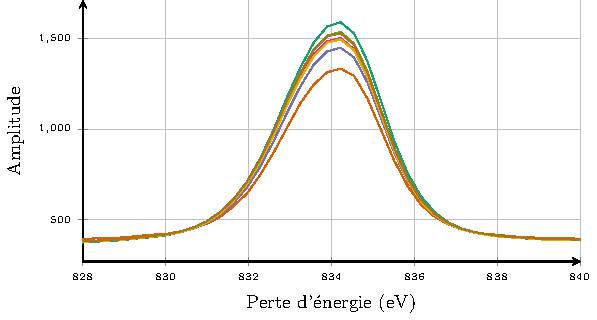
\includegraphics{img/chapitre4/figure6/non-samp-spectrum-zoom.pdf}}\\[0.75cm]
    %
    \caption{Spectres reconstruits pour $\mathsf{R}_2^*$ et pour un pixel non échantillonné dont la position dans l'image est donnée à la figure~\protect\ref{fig-synth-image-spectra-locations}. Les spectres de référence correspondent à l'image non bruitée $\bar{\mathsf{R}}_2$. Le zoom représente la région d'intérêt mise en évidence par la région transparente bleue. Les spectres de NN et 3S sont significativement décalés par rapport à la référence tandis que les spectres reconstruits par CLS et les méthodes par \gls{ad} sont proches du spectre de référence.
        \protect\label{fig-synth-image-spectra}}
\end{normalfigure*}

% Cartes d'erreur
\begin{normalfigure*}[p]
    \centering
    \setlength\tmplength{0.23\textwidth}

\begin{tabular}{m{2cm}*{3}{M{0.24\textwidth}}}
    Masque d'échantillonnage&
    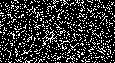
\includegraphics[width=\tmplength]{img/chapitre4/figure9/img/mask.png}&
    &
    \\[30pt]
    %
    Component&
    {$\mathrm{O-K}$}&
    {$\mathrm{La-M}_{4, 5}$}&
    {$\mathrm{Nd-M}_{4, 5}$}\\
    %
    Reference&
    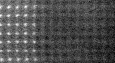
\includegraphics[width=\tmplength]{img/chapitre4/figure7/HR2_GT_band_0.png}&
    
\includegraphics[width=\tmplength]{img/chapitre4/figure7/HR2_GT_band_1.png}&
    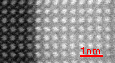
\includegraphics[width=\tmplength]{img/chapitre4/figure7/HR2_GT_band_2.png}\\
    NN&
    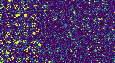
\includegraphics[width=\tmplength]{img/chapitre4/figure7/R2_NN_band_0.png}&
    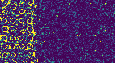
\includegraphics[width=\tmplength]{img/chapitre4/figure7/R2_NN_band_1.png}&
    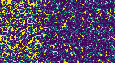
\includegraphics[width=\tmplength]{img/chapitre4/figure7/R2_NN_band_2.png}\\
    3S&
    
\includegraphics[width=\tmplength]{img/chapitre4/figure7/R2_3S_band_0.png}&
    
\includegraphics[width=\tmplength]{img/chapitre4/figure7/R2_3S_band_1.png}&
    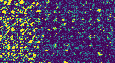
\includegraphics[width=\tmplength]{img/chapitre4/figure7/R2_3S_band_2.png}\\
    CLS&
    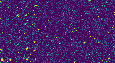
\includegraphics[width=\tmplength]{img/chapitre4/figure7/R2_CLS_band_0.png}&
    
\includegraphics[width=\tmplength]{img/chapitre4/figure7/R2_CLS_band_1.png}&
    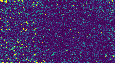
\includegraphics[width=\tmplength]{img/chapitre4/figure7/R2_CLS_band_2.png}\\
    ITKrMM&
    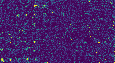
\includegraphics[width=\tmplength]{img/chapitre4/figure7/R2_ITKrMM_band_0.png}&
    
\includegraphics[width=\tmplength]{img/chapitre4/figure7/R2_ITKrMM_band_1.png}&
    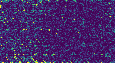
\includegraphics[width=\tmplength]{img/chapitre4/figure7/R2_ITKrMM_band_2.png}\\
    wKSVD&
    
\includegraphics[width=\tmplength]{img/chapitre4/figure7/R2_wKSVD_band_0.png}&
    
\includegraphics[width=\tmplength]{img/chapitre4/figure7/R2_wKSVD_band_1.png}&
    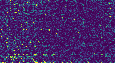
\includegraphics[width=\tmplength]{img/chapitre4/figure7/R2_wKSVD_band_2.png}\\
    BPFA&
    
\includegraphics[width=\tmplength]{img/chapitre4/figure7/R2_BPFA_band_0.png}&
    
\includegraphics[width=\tmplength]{img/chapitre4/figure7/R2_BPFA_band_1.png}&
    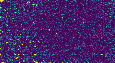
\includegraphics[width=\tmplength]{img/chapitre4/figure7/R2_BPFA_band_2.png}\\
\end{tabular}
    \caption{Erreur de reconstruction pour $\mathsf{R}_2^*$ (NMSE) autour de 3 seuils particuliers ($\mathrm{O-K}$, $\mathrm{La-M}_{4, 5}$ et $\mathrm{Nd-M}_{4, 5}$). La dynamique est la même pour toutes les images, \ie{}, elles peuvent être comparées pour toutes les méthodes et touts les composants. La référence correspond à l'image non bruitée $\bar{\mathsf{R}}_2$.  Le masque d'échantillonnage est aussi donné à la première ligne, où les pixels blanc  correspondent à des pixels échantillonnés.
        \protect\label{fig-results-HR2_synth-bands}}
\end{normalfigure*}

% Histogrammes
\begin{normalfigure*}
    \centering
    \subfigure[Composante $\mathrm{O-K}$]{
        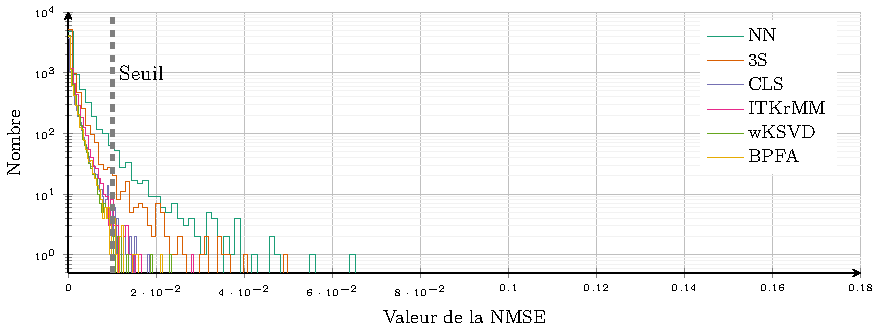
\includegraphics{img/chapitre4/figure8/histogramme_1.pdf}}\\
    \subfigure[Composante $\mathrm{La-M}_{4, 5}$]{
        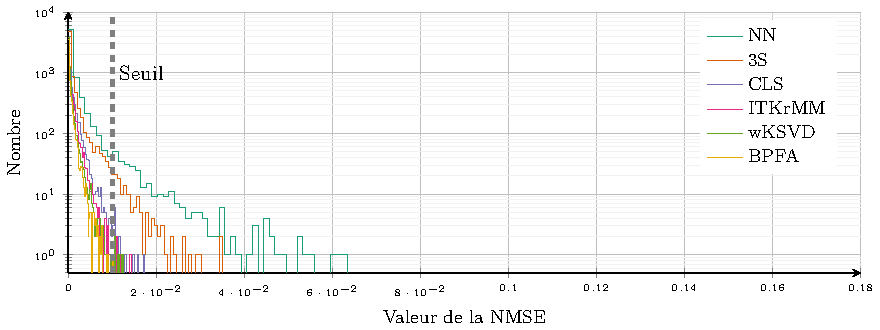
\includegraphics{img/chapitre4/figure8/histogramme_2.pdf}}\\
    \subfigure[Composante $\mathrm{Nd-M}_{4, 5}$]{
        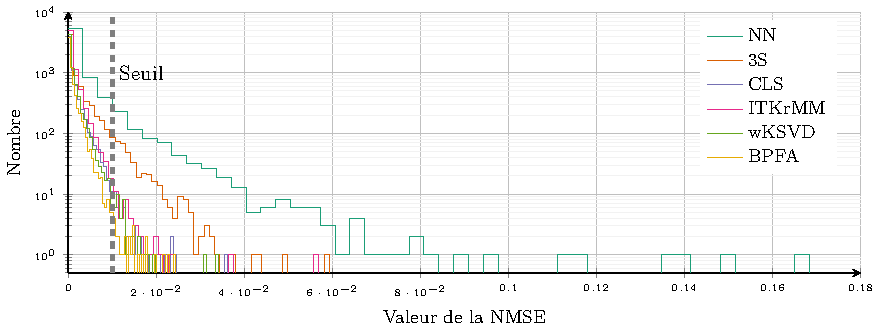
\includegraphics{img/chapitre4/figure8/histogramme_3.pdf}}
    %
    \caption{Histogrammes des erreurs de reconstruction pour $\mathsf{R}_2^*$ en terme de NMSE autour de 3 seuils particuliers ($\mathrm{O-K}$, $\mathrm{La-M}_{4, 5}$ et $\mathrm{Nd-M}_{4, 5}$). Le seuil utilisé pour saturer les images de la figure~\protect\ref{fig-results-HR2_synth-bands} est représenté par une ligne grise en tirets. On observe que les erreurs de NN sont généralement plus grandes que pour les autres méthodes.
        \protect\label{fig-qu1-21-histograms}}    
\end{normalfigure*}


Par conséquence, CLS apparaît comme un compromis pertinent entre précision et complexité puisqu'elle fournit une bonne reconstruction pour un temps d'exécution faible. Cette technique est intéressante comme outil durant l'expérimentation tandis que BPFA peut être utilisée afin de raffiner la reconstruction en post-traitement. Nous verrons à la section~\ref{sec-DL-CLS} comment combiner ces deux approches.



\section{Performances dans le cas de défauts ponctuels}

La présence de défauts ponctuels risque de dégrader les performances de reconstruction pour toutes les méthodes. CLS est censée être impactée puisque sa régularisation favorise la reconstruction d'images périodiques (\cf{} section~\ref{sec-formulation-cls}). \`A l'inverse, les méthodes par \gls{ad} devraient souffrir de la faible  représentation du défaut ponctuel dans l'échantillon. En effet, si le défaut ponctuel est rare, il est peu probable que les atomes appris puissent le représenter de manière parcimonieuse.

Afin d'illustrer cet impact, un nouveau spectre-image synthétique noté $\mathsf{S}_v^*$ a été généré de même que pour l'image $\mathsf{S}^*$, mis à part que deux atomes initialement situés des deux côtés de l'interface ont été échangés. Cela permet d'imiter la présence d'un défaut ponctuel.

La \tabname~\ref{table-vacancy-perfs} expose les performances de reconstruction obtenues pour les images $\mathsf{S}^*$ et $\mathsf{S}_v^*$. Les figures~\ref{fig-vacancy-S} et \ref{fig-vacancy-SV} montrent les cartes d'erreur en NMSE associées aux deux images $\mathsf{S}^*$ et $\mathsf{S}_v^*$ respectivement, calculées autour de trois seuils d'intérêt. On observe que NN et 3S ne sont pas impactées par la présence de défauts ponctuels. Cependant, les performances de CLS et des techniques par \gls{ad}, en particulier \gls{itkrmm}, sont dégradées. Cette dégradation est particulièrement visible dans les cartes d'erreur associées au composant $\mathrm{La-M}_{4, 5}$. On observe que les erreurs de NN et 3S sont globalement les mêmes  pour tous les atomes tandis que, pour les méthodes CLS et par \gls{ad}, les erreurs sont localisées autour des défauts ponctuels.

Pour conclure, dans le cas de défauts ponctuels, les performances de CLS, bien que dégradées, ne semblent pas moins sensibles que les techniques par \gls{ad}.

\begin{normalfigure*}[]
    \centering
    %
    \begin{tabular}{m{0.12\textwidth}*{3}{M{0.21\textwidth}}}
Composant&O - K&La - M\textsubscript{4, 5}&Nd - M\textsubscript{4, 5}\\
Référence
&
\includegraphics[width=0.2\textwidth]{img/chapitre4/figure15/synth/Synth_GT_band_0.png}
&
\includegraphics[width=0.2\textwidth]{img/chapitre4/figure15/synth/Synth_GT_band_1.png}
&
\includegraphics[width=0.2\textwidth]{img/chapitre4/figure15/synth/Synth_GT_band_2.png}
\\
PPV
&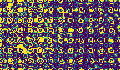
\includegraphics[width=0.2\textwidth]{img/chapitre4/figure15/synth/Synth_interpolation_band_0.png}
&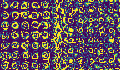
\includegraphics[width=0.2\textwidth]{img/chapitre4/figure15/synth/Synth_interpolation_band_1.png}
&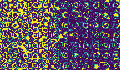
\includegraphics[width=0.2\textwidth]{img/chapitre4/figure15/synth/Synth_interpolation_band_2.png}
\\
3S
&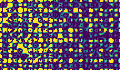
\includegraphics[width=0.2\textwidth]{img/chapitre4/figure15/synth/Synth_3S_band_0.png}
&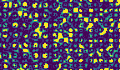
\includegraphics[width=0.2\textwidth]{img/chapitre4/figure15/synth/Synth_3S_band_1.png}
&\includegraphics[width=0.2\textwidth]{img/chapitre4/figure15/synth/Synth_3S_band_2.png}
\\
CLS
&\includegraphics[width=0.2\textwidth]{img/chapitre4/figure15/synth/Synth_CLS_band_0.png}
&\includegraphics[width=0.2\textwidth]{img/chapitre4/figure15/synth/Synth_CLS_band_1.png}
&\includegraphics[width=0.2\textwidth]{img/chapitre4/figure15/synth/Synth_CLS_band_2.png}
\\
ITKrMM
&\includegraphics[width=0.2\textwidth]{img/chapitre4/figure15/synth/Synth_ITKrMM_matlab_band_0.png}
&\includegraphics[width=0.2\textwidth]{img/chapitre4/figure15/synth/Synth_ITKrMM_matlab_band_1.png}
&\includegraphics[width=0.2\textwidth]{img/chapitre4/figure15/synth/Synth_ITKrMM_matlab_band_2.png}
\\
wKSVD
&\includegraphics[width=0.2\textwidth]{img/chapitre4/figure15/synth/Synth_wKSVD_matlab_band_0.png}
&\includegraphics[width=0.2\textwidth]{img/chapitre4/figure15/synth/Synth_wKSVD_matlab_band_1.png}
&\includegraphics[width=0.2\textwidth]{img/chapitre4/figure15/synth/Synth_wKSVD_matlab_band_2.png}
\\
BPFA
&\includegraphics[width=0.2\textwidth]{img/chapitre4/figure15/synth/Synth_BPFA_matlab_band_0.png}
&\includegraphics[width=0.2\textwidth]{img/chapitre4/figure15/synth/Synth_BPFA_matlab_band_1.png}
&\includegraphics[width=0.2\textwidth]{img/chapitre4/figure15/synth/Synth_BPFA_matlab_band_2.png}
\\
\end{tabular} 
    %
    \caption{Erreur de reconstruction pour $\mathsf{S}^*$ (NMSE) autour de trois seuils d'intérêt ($\mathrm{O-K}$, $\mathrm{La-M}_{4, 5}$ et $\mathrm{Nd-M}_{4, 5}$). La dynamique est la même pour toutes les images, \ie{}, elles peuvent être comparées pour toutes les méthodes et tous les composants. Les bandes du spectre-image synthétique de référence sont aussi données pour comparaison à la première ligne.
        \protect\label{fig-vacancy-S}}
\end{normalfigure*}

\begin{normalfigure*}[]
    \centering
    %
    \begin{tabular}{m{0.12\textwidth}*{3}{M{0.21\textwidth}}}
Component&O - K&La - M\textsubscript{4, 5}&Nd - M\textsubscript{4, 5}\\
Reference
&\includegraphics[width=0.2\textwidth]{img/chapitre4/figure15/synth_hole/SynthH_GT_band_0.png}
&\includegraphics[width=0.2\textwidth]{img/chapitre4/figure15/synth_hole/SynthH_GT_band_1.png}
&\includegraphics[width=0.2\textwidth]{img/chapitre4/figure15/synth_hole/SynthH_GT_band_2.png}
\\
NN
&\includegraphics[width=0.2\textwidth]{img/chapitre4/figure15/synth_hole/SynthH_interpolation_band_0.png}
&\includegraphics[width=0.2\textwidth]{img/chapitre4/figure15/synth_hole/SynthH_interpolation_band_1.png}
&\includegraphics[width=0.2\textwidth]{img/chapitre4/figure15/synth_hole/SynthH_interpolation_band_2.png}
\\
3S
&\includegraphics[width=0.2\textwidth]{img/chapitre4/figure15/synth_hole/SynthH_3S_band_0.png}
&\includegraphics[width=0.2\textwidth]{img/chapitre4/figure15/synth_hole/SynthH_3S_band_1.png}
&\includegraphics[width=0.2\textwidth]{img/chapitre4/figure15/synth_hole/SynthH_3S_band_2.png}
\\
CLS
&\includegraphics[width=0.2\textwidth]{img/chapitre4/figure15/synth_hole/SynthH_CLS_band_0.png}
&\includegraphics[width=0.2\textwidth]{img/chapitre4/figure15/synth_hole/SynthH_CLS_band_1.png}
&\includegraphics[width=0.2\textwidth]{img/chapitre4/figure15/synth_hole/SynthH_CLS_band_2.png}
\\
ITKrMM
&\includegraphics[width=0.2\textwidth]{img/chapitre4/figure15/synth_hole/SynthH_ITKrMM_matlab_band_0.png}
&\includegraphics[width=0.2\textwidth]{img/chapitre4/figure15/synth_hole/SynthH_ITKrMM_matlab_band_1.png}
&\includegraphics[width=0.2\textwidth]{img/chapitre4/figure15/synth_hole/SynthH_ITKrMM_matlab_band_2.png}
\\
wKSVD
&\includegraphics[width=0.2\textwidth]{img/chapitre4/figure15/synth_hole/SynthH_wKSVD_matlab_band_0.png}
&\includegraphics[width=0.2\textwidth]{img/chapitre4/figure15/synth_hole/SynthH_wKSVD_matlab_band_1.png}
&\includegraphics[width=0.2\textwidth]{img/chapitre4/figure15/synth_hole/SynthH_wKSVD_matlab_band_2.png}
\\
BPFA
&\includegraphics[width=0.2\textwidth]{img/chapitre4/figure15/synth_hole/SynthH_BPFA_matlab_band_0.png}
&\includegraphics[width=0.2\textwidth]{img/chapitre4/figure15/synth_hole/SynthH_BPFA_matlab_band_1.png}
&\includegraphics[width=0.2\textwidth]{img/chapitre4/figure15/synth_hole/SynthH_BPFA_matlab_band_2.png}
\\
\end{tabular}
    %
    \caption{Erreur de reconstruction pour $\mathsf{S}_v^*$ (NMSE) autour de trois seuils d'intérêt ($\mathrm{O-K}$, $\mathrm{La-M}_{4, 5}$ et $\mathrm{Nd-M}_{4, 5}$). La dynamique est la même pour toutes les images, \ie{}, elles peuvent être comparées pour toutes les méthodes et tous les composants. Les bandes du spectre-image synthétique de référence sont aussi données pour comparaison à la première ligne. La présence de défauts ponctuels dégrade les performances de reconstruction de CLS et des méthodes par \gls{ad}.
        \protect\label{fig-vacancy-SV}}
\end{normalfigure*}

\begin{normaltable*}[p]
    \centering
    \begin{tabular}{c*{6}{M{2cm}}}
        \toprule
        \multirow{2}*{Méthode}&
        \multicolumn{3}{c}{Sans défaut ponctuel}&
        \multicolumn{3}{c}{Avec défaut ponctuel}\\
        &SNR&aSAD (100$\times$)&SSIM&SNR&aSAD (100$\times$)&SSIM\\
        \midrule
        NN      &21,32  &1,462  &0,735  &21,32  &1,475  &0,738\\
        3S      &22,12  &1,174  &0,710  &22,13  &1,181  &0,715\\
        CLS     &42,14  &0,224  &0,997  &38,45  &0,346  &0,993\\
        ITKrMM  &44,16  &0,338  &0,998  &34,34  &0,649  &0,987\\
        \gls{wksvd}   &45,59  &0,277  &0,999  &41,49  &0,376  &0,997\\
        BPFA    &52,70  &0,150  &1,000  &45,27  &0,236  &0,998\\
        \bottomrule    
    \end{tabular}
    \caption{Performances de reconstruction avec et sans défaut ponctuel.
        \protect\label{table-vacancy-perfs}}
\end{normaltable*}



\subsection{Résultats sur données réelles}

Des résultats illustratifs sont également donnés pour $\mathbf{R}_2$. Plus précisément, le spectre-image réel $\mathbf{R}_2$ est spatialement sous-échantillonné avec un taux d'échantillonnage de 20\%, puis reconstruit comme à la section précédente~\ref{sec-results-hr-synth}.

Des représentations visuelles des spectre-images reconstruits autour de seuils d'intérêt sont données à la figure~\ref{fig-results-HR2_real-bands} et la reconstruction d'un spectre non échantillonné est montrée à la figure~\ref{fig-real-image-spectra}. Dans ces figures, notons que les données de référence correspondent à l'image réelle $\mathsf{R}_2$ possiblement bruitée.

Comme précédemment observé, les méthodes par \gls{ad} donnent des images reconstruites visuellement excellentes comparé aux autres méthodes. Les résultats concernant les spectres reconstruits montrent que le spectre reconstruit par NN pour un pixel non-acquis souffre d'un décalage significatif tandis que les autres algorithmes font preuve de biais bien moins prononcés. 


\begin{normalfigure*}[]
    \centering
    \setlength\tmplength{0.23\textwidth}

\begin{tabular}{m{2cm}*{3}{M{0.24\textwidth}}}
    Masque d'échantillonnage&
    \includegraphics[width=\tmplength]{img/chapitre4/figure9/img/mask.png}&
    &
    \\[30pt]
    %
    Composant&
    {$\mathrm{O-K}$}&
    {$\mathrm{La-M}_{4, 5}$}&
    {$\mathrm{Nd-M}_{4, 5}$}\\
    %
    Référence&
    \includegraphics[width=\tmplength]{img/chapitre4/figure9/img/GT_band_0.png}&
    \includegraphics[width=\tmplength]{img/chapitre4/figure9/img/GT_band_1.png}&
    \includegraphics[width=\tmplength]{img/chapitre4/figure9/img/GT_band_2.png}\\
    NN&
    \includegraphics[width=\tmplength]{img/chapitre4/figure9/img/NN_band_0.png}&
    \includegraphics[width=\tmplength]{img/chapitre4/figure9/img/NN_band_1.png}&
    \includegraphics[width=\tmplength]{img/chapitre4/figure9/img/NN_band_2.png}\\
    3S&
    \includegraphics[width=\tmplength]{img/chapitre4/figure9/img/SSS_band_0.png}&
    \includegraphics[width=\tmplength]{img/chapitre4/figure9/img/SSS_band_1.png}&
    \includegraphics[width=\tmplength]{img/chapitre4/figure9/img/SSS_band_2.png}\\
    CLS&
    \includegraphics[width=\tmplength]{img/chapitre4/figure9/img/FS3D_band_0.png}&
    \includegraphics[width=\tmplength]{img/chapitre4/figure9/img/FS3D_band_1.png}&
    \includegraphics[width=\tmplength]{img/chapitre4/figure9/img/FS3D_band_2.png}\\
    ITKrMM&
    \includegraphics[width=\tmplength]{img/chapitre4/figure9/img/ITKrMM_band_0.png}&
    \includegraphics[width=\tmplength]{img/chapitre4/figure9/img/ITKrMM_band_1.png}&
    \includegraphics[width=\tmplength]{img/chapitre4/figure9/img/ITKrMM_band_2.png}\\
    wKSVD&
    \includegraphics[width=\tmplength]{img/chapitre4/figure9/img/wKSVD_band_0.png}&
    \includegraphics[width=\tmplength]{img/chapitre4/figure9/img/wKSVD_band_1.png}&
    \includegraphics[width=\tmplength]{img/chapitre4/figure9/img/wKSVD_band_2.png}\\
    BPFA&
    \includegraphics[width=\tmplength]{img/chapitre4/figure9/img/BPFA_band_0.png}&
    \includegraphics[width=\tmplength]{img/chapitre4/figure9/img/BPFA_band_1.png}&
    \includegraphics[width=\tmplength]{img/chapitre4/figure9/img/BPFA_band_2_size.png}\\
\end{tabular}
    \caption{Résultats de reconstruction pour $\mathbf{R}_2$. Les images montrent la somme de 5 bandes autour de trois seuils particuliers ($\mathrm{O-K}$, $\mathrm{La-M}_{4, 5}$ et $\mathrm{Nd-M}_{4, 5}$). 
    %
    Ces résultats confirment l'écart de performances entre NN dont les images ne sont pas assez lisses et les méthodes par \gls{ad} qui sont proches de la référence avec un effet additionnel de débruitage. Les résultats de CLS sont clairement meilleurs que NN et 3S et sont proches des résultats pour les méthodes par \gls{ad}. 
        \protect\label{fig-results-HR2_real-bands}}
\end{normalfigure*}


\begin{normalfigure*}[]
    \centering
    \subfigure[Pixel non-acquis]{
        \includegraphics{img/chapitre4/figure10/non-samp-spectrum.pdf}}\\[0.75cm]
    \subfigure[Pixel non-acquis (zoom)]{
        \includegraphics{img/chapitre4/figure10/non-samp-spectrum-zoom.pdf}}\\[0.75cm]
    %
    \caption{Spectres résultant de la reconstruction de $\mathsf{R}_2$ pour un spectre non échantillonné avec la même position que celle de la figure~\protect\ref{fig-synth-image-spectra}. Le spectre de référence correspond à l'image réelle $\mathsf{R}_2$. Le zoom représente la région d'intérêt mise en évidence par la région transparente bleue. Comme pour les résultats synthétiques, le spectre reconstruit par NN est significativement décalé comparé au spectre de référence tandis que les résultats pour CLS et les méthodes par \gls{ad} (tout particulièrement BPFA) sont proches de la référence. Encore, CLS apparaît comme un compromis pertinent.
        \protect\label{fig-real-image-spectra}}
\end{normalfigure*}

 
\subsection{Résultats des approches DL-CLS}\label{sec-DL-CLS}

Les sections précédentes ont comparés les performances de reconstruction en se basant sur des images synthétique, semi-réelles et réelles. elles ont illustré l'intérêt de CLS en tant que méthode à la fois rapide et efficace pour reconstruire un spectre-image sous-échantillonné de réseau cristallin périodique. De plus, les méthodes de reconstruction par \gls{ad} ont affiché des performances meilleures pour une charge de calcul plus grande. Toutefois, une fois couplées à CLS, ces méthodes pourraient être utilisées comme raffinement après l'expérimentation. 
%
Dans cette section, cet intérêt sera confirmé en se basant sur des expériences additionelles conduites sur l'image semi-réelle $\mathsf{R}_2^*$. De manière similaire à la section~\ref{sec-results-hr-synth}, cette image a été sous-échantillonnée, puis reconstruite avec \gls{wksvd} en considérant deux initialisations distinctes. 
%
La première est purement aléatoire, comme cela a été initialement implémenté par l'algorithme. La seconde initialisation consiste à initialiser \gls{wksvd} avec un dictionnaire et un code parcimonieux associé obtenu à partir de l'image reconstruite par CLS. 
%
Pour comparer les deux initialisations, la qualité de reconstruction (SNR) est évaluée à chaque itération de l'algorithme pour les deux initialisations. Les résultats sont donnés à la figure~\ref{fig-FS_init}. 
%
%Ensuite, la qualité de reconstruction est suivie comme une fonction de l'itération de l'algorithme \gls{wksvd} en affichant le SNR lié à la reconstruction. Les résultats sont donnés à la figure~\ref{fig-FS_init} pour les deux initialisations.

\begin{figure}[htbp]
   \centering
   \includegraphics{img/chapitre4/figure11/CLS_init.pdf}
   \caption{SNR en fonction de l'itération de \gls{wksvd} pour les initialisations aléatoires et basées sur CLS. Les régions colorées correspondent à l'intervalle de l'écart-type calculé pour $10$ réalisations. Les résultats montrent que l'initialisation par CLS nécessite moins d'itérations pour atteindre un SNR désiré comparé à l'initialisation aléatoire. Cela encourage l'utilisation de CLS pour initialiser des techniques de reconstruction par \gls{ad}.
       \protect\label{fig-FS_init}}
\end{figure}


Les résultats montrent que l'initialisation basée sur CLS nécessite moins d'itérations pour parvenir à un SNR souhaité comparé à l'initialisation aléatoire. De plus, il semble même qu'à convergence, les performances soient améliorées.
%
Cela confirme l'intérêt à utiliser CLS en vue d'élaborer une initialisation pertinente pour accélérer des techniques plus élaborées mais plus lourdes d'un point de vue calculatoire.  Notons que cette stratégie peut être utilisée pour des algorithmes basés sur une descente de gradient, tels que \gls{wksvd} ou ITKrMM, mais ne convient pas aux méthodes de \gls{mcmc} comme BPFA.


%
\section{Conclusion}

Dans ce chapitre, une nouvelle méthode de reconstruction d'images STEM-EELS nommée CLS a été proposée. Des expériences conduites sur des données synthétiques et réelles ont montré qu'elle était bien plus rapide que les méthodes par \gls{ad} et plus précise que NN. La combinaison de ces deux avantages est particulièrement intéressante et permet d'envisager son intégration dans une configuration expérimentale en ligne.

De plus, des techniques par \gls{ad} plus coûteuses mais plus précises ont été aussi utilisées comme post-traitement des résultats fournis par CLS. 
%
Ces méthodes donnent des reconstructions d'excellente qualité au prix d'un temps d'exécution élevé, pouvant être réduit en initialisant l'algorithme avec le spectre-image obtenu par CLS.

Mener une acquisition sur un microscope tout en reconstruisant l'image en ligne est un domaine de recherche très actif puisque cela accélère la procédure d'acquisition et l'identification des composantes. Réaliser une reconstruction en ligne avec CLS et le coupler avec une acquisition adaptative est une perspective intéressante vers l'imagerie dynamique en STEM-EELS. Un tel protocole d'acquisition permettrait d'observer l'évolution temporelle de l'échantillon.


% e gérer la dérive de l'échantillon, ce qui n'a pas été le cas des expériences menées dans ce chapitre.


